% Created 2019-05-20 Mon 15:14
% Intended LaTeX compiler: xelatex
\documentclass[11pt]{article}
\usepackage{graphicx}
\usepackage{grffile}
\usepackage{longtable}
\usepackage{wrapfig}
\usepackage{rotating}
\usepackage[normalem]{ulem}
\usepackage{amsmath}
\usepackage{textcomp}
\usepackage{amssymb}
\usepackage{capt-of}
\usepackage{hyperref}
\usepackage{float}
\usepackage{indentfirst}
\setlength{\parindent}{2.0cm}
\usepackage[utf8]{inputenc}
\usepackage[T1]{fontenc}
\usepackage{lipsum}
\usepackage{mwe}
\usepackage{lmodern}
\usepackage{graphicx}
\usepackage{caption}
\usepackage{floatrow}
\usepackage[super,square,comma,sort&compress]{natbib}
\usepackage[UTF8]{ctex}
\setCJKmainfont{Source Han Serif CN}
\author{Wei Guan,Fangying Jin,Qingkong Chen,Peng Yan,Qian Zhang}
\date{}
\title{多孔硅的制备及磷回收性能\\\medskip
\large 硅酸钙水合物}
\hypersetup{
 pdfauthor={Wei Guan,Fangying Jin,Qingkong Chen,Peng Yan,Qian Zhang},
 pdftitle={多孔硅的制备及磷回收性能},
 pdfkeywords={},
 pdfsubject={},
 pdfcreator={Emacs 26.2 (Org mode 9.2.2)}, 
 pdflang={English}}
\begin{document}

\maketitle
\tableofcontents

\noindent\rule{\textwidth}{0.5pt}
\begin{abstract}


多孔硅酸钙水合物用于从废水中合成并回收磷。本研究的主要目的是探讨由不同的$Ca/Si$摩尔比制备的多孔硅酸钙水合物的磷回收性能。也通过场发射扫描电子显微镜($FESEM$),能量色散谱($EDS$),布鲁诺-埃梅特-特勒($BET$)和X射线衍射($XRD$)研究磷回收机制。$Ca^{2+}$的释放规律是磷回收性能的关键。不同的$Ca/Si$摩尔比导致孔隙结构的变化。比表面积的增加和$Ca^{2+}$释放浓度的增加相一致。多孔硅酸钙-水合物的$Ca/Si$摩尔比为$1.6$时更适合回收磷。多孔硅酸钙水合物的孔结构提供了维持高浓度$Ca^{2+}$释放的局部条件。多孔硅酸钙水合物可以释放适当浓度的$Ca^{2+}$和$OH$,使pH值保持在$8.5-9.5$。这种条件有利于羟基磷灰石的形成。磷回收后,多孔硅酸钙水合物的磷含量达到$18.64%$。


{{\it keywords:} 硅酸钙水合物; 磷回收; 多孔结构; 制备}}

\end{abstract}

\noindent\rule{\textwidth}{0.5pt}

\section{简介}
\label{sec:org1f5286c}
磷不仅在水体富营养化中起着重要作用,而且是一种不可再生和不可替代的资源。cite:Suzuki\textsubscript{2007} 全球磷
矿资源将在100年内完全耗尽。因此,废水回收被认为是开发可持续磷资源的唯一途径。
cite:Efficiency\textsubscript{and}\textsubscript{mechanism}\textsubscript{of}\textsubscript{phosphorus}\textsubscript{removal}\textsubscript{by}\textsubscript{coagulation}\textsubscript{of}\textsubscript{iron}\textsubscript{manganese}\textsubscript{composited}\textsubscript{oxide,song07}\textsubscript{seed}\textsubscript{selec}\textsubscript{cryst}\textsubscript{calcium}\textsubscript{phosp}\textsubscript{phosp}\textsubscript{recov}
以羟基磷灰石形式从废水中回收磷是一种常见且简单的方法。
cite:chen09\textsubscript{phosp}\textsubscript{remov}\textsubscript{recov}\textsubscript{throug}\textsubscript{cryst,muench01}\textsubscript{contr}\textsubscript{struv}\textsubscript{cryst}\textsubscript{remov}\textsubscript{phosp,song06}\textsubscript{calcit}\textsubscript{seeded}\textsubscript{cryst}\textsubscript{calcium}\textsubscript{phosp}\textsubscript{phosp}\textsubscript{recov}
然而,在羟基磷灰石的形成
过程中,超饱和是一种常见现象。羟基磷灰石形成的最佳pH值范围为10.5-12.5 cite:liu03\textsubscript{influen}\textsubscript{ph}\textsubscript{temper}\textsubscript{morph}\textsubscript{hydrox} 这个pH
值太高,生化处理系统的pH值在6.0到9.0之间。cite:hood01\textsubscript{bioch}\textsubscript{hypot}\textsubscript{explain}\textsubscript{respon}\textsubscript{enhan} 对于通过化学方法辅助的生物处理过程去
除磷,较高的pH值也增加了碳酸盐和钙之间的显着竞争。cite:battistoni00\textsubscript{struv}\textsubscript{cryst}
同时,化学处理成本增加,最终产品的有效磷组分减少。cite:sengupta11\textsubscript{selec}\textsubscript{remov}\textsubscript{phosp}\textsubscript{from}\textsubscript{wastew}

硅酸钙-水合物(CSH)作为晶种可用于通过羟基磷灰石结晶去除废
水中的磷。cite:battistoni01\textsubscript{phosp}\textsubscript{remov}\textsubscript{from}\textsubscript{real}\textsubscript{anaer} Ca\textsuperscript{2+}和OH\textsuperscript{-}从CSH中释放出来并在pH = 8.5-9.5的条件下与磷酸盐反应生成羟基
磷灰石。然而,在实际应用中,CSH的磷含量太低而不能回收磷。
cite:renman10\textsubscript{long}\textsubscript{term}\textsubscript{phosp}\textsubscript{remov}\textsubscript{by,de}-bashan04\textsubscript{recen}\textsubscript{advan}\textsubscript{remov}\textsubscript{phosp}\textsubscript{from}  Ca\textsuperscript{2+}和OH\textsuperscript{-}的释放效率与
CSH cite:yin11\textsubscript{phosp}\textsubscript{remov}\textsubscript{from}\textsubscript{wastew}\textsubscript{by} 的孔结构有关,影响磷的回收性能。
cite:westholm06\textsubscript{subst}\textsubscript{phosp}\textsubscript{remov}\textsubscript{poten}\textsubscript{benef,baur04}\textsubscript{dissol}\textsubscript{precip}\textsubscript{behav}\textsubscript{ettrin}\textsubscript{monos}
Ca/Si摩尔比对CSH
cite:chen04\textsubscript{solub}\textsubscript{struc}\textsubscript{calcium}\textsubscript{silic}\textsubscript{hydrat,soyer}-uzun11\textsubscript{compos}\textsubscript{evolut}\textsubscript{calcium}\textsubscript{silic}\textsubscript{hydrat,richardson04}\textsubscript{tober}\textsubscript{tober}\textsubscript{hydrox}\textsubscript{based}\textsubscript{model}
的孔结构具有显着影响。在磷回
收性能方面,尚未确定Ca/Si摩尔比与磷回收性能之间的系统关系。Ca/Si摩尔比对磷回收性
能影响的机理以及Ca\textsuperscript{2+}和OH\textsuperscript{-}释放规律尚不清楚。因此,确定CSH的适当Ca/Si摩尔比以回收磷是一项挑战。

该研究的主要目的是找到适当的CSH回收磷的Ca/Si的摩尔比。本文的原创性和重要性由以下三点强调:
\begin{enumerate}
\item 采用动态水热法,采用碳化物残渣和白炭黑合成了多孔硅酸钙水合物。 cite:li04\textsubscript{format}\textsubscript{micro}\textsubscript{porous}\textsubscript{spher}\textsubscript{partic,mansur10}\textsubscript{prepar}\textsubscript{charac}\textsubscript{cytoc}\textsubscript{bioac}\textsubscript{coatin} 研究了Ca/Si摩尔比对磷回收性能的影响。
\item 通过Avrami动力学模型建立了孔隙结构与Ca\textsuperscript{2+}和OH\textsuperscript{-}释放规律之间的关系。
\item 在深入研究的基础上,通过FESEM,EDS,BET和XRD研究了磷的回收机理。
\end{enumerate}

\section{材料和方法}
\label{sec:orgdf89ce5}
\subsection{多孔硅酸钙水合物的制备}
\label{sec:org5675872}
用碳化物残余物(提供Ca)和白炭黑(提供Si)合成多孔硅酸钙水合物。碳化物残渣(钙
质,灰白和粉末)从重庆长寿化学有限公司获得,并在700℃下煅烧2小时。白炭黑(粒径均
匀的球形颗粒)购自重庆建峰化工有限公司。碳化物残渣和白炭黑的化学成分见表1。雪硅钙
石(化学式Ca\textsubscript{5}Si\textsubscript{6}O\textsubscript{16}(OH)\textsubscript{2} \dot 7H\textsubscript{2}O;理论Ca/Si 摩尔比为0.83),一种硅酸钙水合物,购自Hdlapp and Ratus(Shanghai)Co.Ltd.,通过加入KH\textsubscript{2}PO\textsubscript{4}(分析试剂,重庆博依化学试剂有限公司)调节磷溶液。制备初始磷浓度为100mg/L的溶液。将上述材料和化学品放入密封瓶中储存。

混合碳化物残渣和白炭黑,Ca/Si摩尔比控制在0.6,1.0,1.6和2.2。然后将混合物加入到
制备的浆料中。将浆料在170℃下水热反应6小时,并在温度降至自然条件时取出。水热反应
在液/固比为30的条件下进行。所得产物在105℃下干燥2小时,然后通过200目的筛子研磨。
将Ca/Si摩尔比为0.6, 1.0 ,1.6和2.2的制备样品分别表示为CSH: Ca/Si = 0.6,CSH: Ca/Si
= 1.0,CSH: Ca/Si = 1.6和CSH: Ca/Si = 2.2。
\subsection{评估磷回收性能}
\label{sec:org537a8b6}
将合成溶液(1L)分别加入瓶中。将一定质量的样品(500,1000,2000,3000,4000,5000和
6000mg)分别加入这些瓶中,并在受控温度条件(20℃)下以40r/min摇动。使用Unico分
光光度计(UV 2102PCS,Shanghai Unico Instruments Co.,Ltd.,中国),
cite:gustafsson08\textsubscript{phosp}\textsubscript{remov}\textsubscript{by}\textsubscript{miner}\textsubscript{based} 根据钼 - 蓝抗坏血酸法(数据的相对
误差为0.3\%)测量上清液的磷浓度。然后将反应后的固体样品与除去的合成溶液分离,并再
次加入初始磷浓度为100mg/L的合成溶液中。重复该实验数次,直到加入样品使磷浓度保持不
变。最后,将产生的沉淀物与除去的合成溶液分离,干燥并称重。通过方程式计算磷回收后的
样品的磷含量(P)。式(1)中Ct是合成溶液中的限制磷浓度(mg/L),v是溶液的体积(L),w是磷回收后产生的沉积物的质量(mg),C\textsubscript{0}是初始磷浓度(mg/L)。

\[P = \frac{(c_{0} - c_{t})v}{w} 100\% \ \ \  (1)\]

将4g样品(CSH: Ca/Si = 0.6,CSH: Ca/Si = 1.0,CSH: Ca/Si = 1.6,CSH: Ca/Si = 2.2和雪硅钙石)浸入分别包含在其中的1L去离子水中。一个玻璃瓶,生成溶液浓度为4克/升的样品。将瓶子放在搅拌台上并在控制温度条件(20℃)下以40r/min摇动。在搅拌5,10,15,20,40,60,80和100分钟后取出溶液样品。通过EDTA滴定测定样品的Ca\textsuperscript{2+}浓度(数据的相对误差为0.05\%)。cite:kim03\textsubscript{effec}\textsubscript{ph}\textsubscript{sulfat}\textsubscript{sodium}\textsubscript{edta}\textsubscript{titrat}\textsubscript{calcium}

\noindent\rule{\textwidth}{0.5pt}

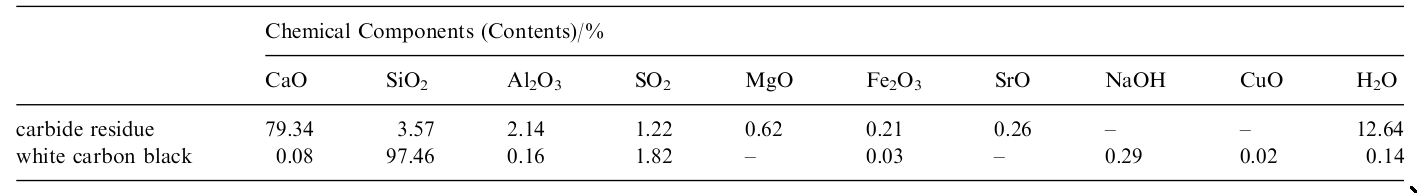
\includegraphics[width=0.9\textwidth]{table.1.new.png}
\captionof{table}{碳化物残基和白炭黑的化学成分} \label{tab:title}

\noindent\rule{\textwidth}{0.5pt}

\subsection{表征方法}
\label{sec:org65ad314}
\setlength{\parindent}{1.0cm}
使用CuKα辐射在XD-2仪器(Persee,China)中收集XRD图案。在S-4800场发射扫描电子显微镜(日立,日本)上收集FESEM图像。在ASAP-2010吸附装置(Micromeritics,USA)上通过氮吸附在77.35K下测量BET表面积。
\par
\section{结果和讨论}
\label{sec:org908a915}
\subsection{多孔硅酸钙水合物的磷回收性能}
\label{sec:orgac4ab57}
\setlength{\parindent}{1.0cm}
反应时间对抑制磷浓度的影响如图1所示。在最初的20分钟内观察到磷浓度急剧下降。随着时间的延长,磷浓度略有下降。当反应在60分钟达到平衡时,抑制磷浓度的差异是显着的。当Ca/Si摩尔比为0.6时,抑制磷浓度达到22.19mg/L。随着Ca/Si摩尔比的增加,样品的除磷能力显着提高。当Ca/Si摩尔比为2.2时,抑制磷浓度为2.16mg/L。
\par

\setlength{\parindent}{1.0cm}
图2显示了不同样品投加的磷去除。当剂量增加时,磷去除效率提高,并且在4000mg/L时获
得最高的去除效率。然后,随着样品剂量的进一步增加,除磷效率几乎保持稳定。相比较而
言,CSH: Ca/Si = 2.2显示出最高的除磷效率。限制磷浓度仅为2.16mg/L,沉积物质量为
3750mg。但是,CSH: Ca/Si = 2.2的磷含量仅为2.6\%。由于磷的去除循环,样品的磷含量可以增加。
\par


\noindent\rule{\textwidth}{0.5pt}

\begin{figure}
    \centering
    \begin{minipage}{0.45\textwidth}
        \centering
        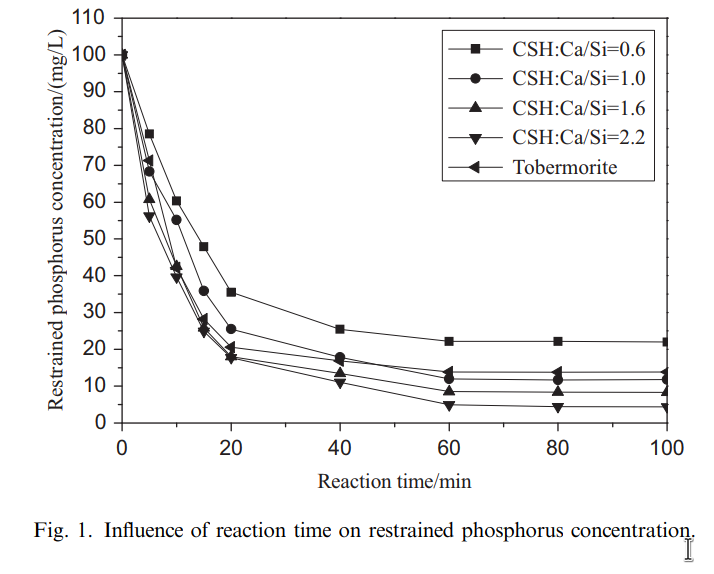
\includegraphics[width=0.9\textwidth]{fig.1.png} % first figure itself
        \caption{反应时间对抑制磷浓度的影响}
    \end{minipage}\hfill
    \begin{minipage}{0.45\textwidth}
        \centering
        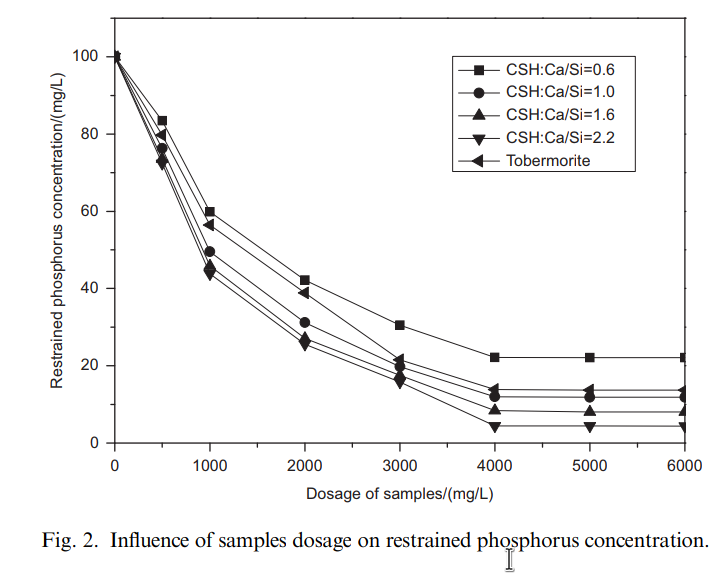
\includegraphics[width=0.9\textwidth]{fig.2.png} % second figure itself
        \caption{样品用量对抑制磷浓度的影响}
    \end{minipage}
\end{figure}


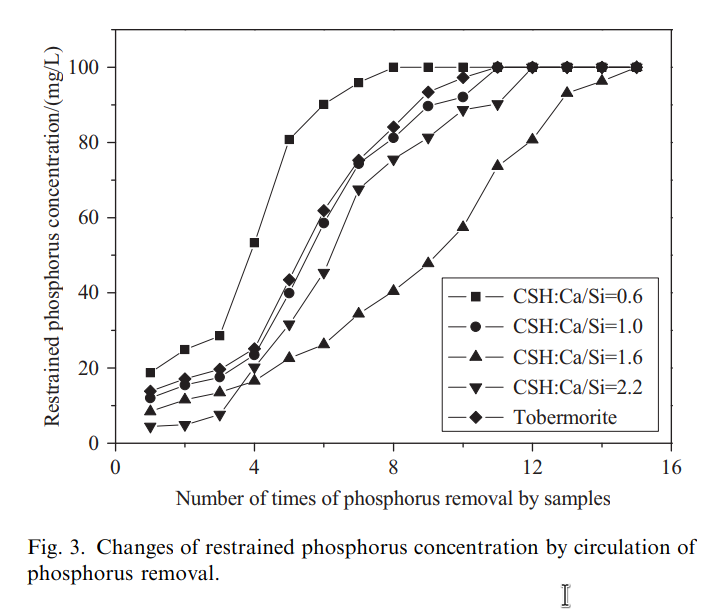
\includegraphics[width=0.9\textwidth]{fig.3.png}
\captionof{figure}{除磷循环抑制磷浓度的变化} \label{tab:title}

\noindent\rule{\textwidth}{0.5pt}



\setlength{\parindent}{1.0cm}
从除去的合成溶液中分离样品,然后加入初始磷浓度为100mg/L的合成溶液中。抑制磷浓度
的变化如图3所示。CSH的除磷性能: Ca/Si = 2.2在前3次保持良好,在第12次后停止。
CSH: Ca/Si = 2.2的磷含量为14.10\%,而CSH: Ca/Si = 1.6的磷含量达到18.64\%。CSH:与
CSH相比,Ca/Si = 1.6具有更高的磷回收性能: Ca/Si = 2.2.样品的磷去除性能与pH值有关。随着磷去除时间的延长,pH值降低(图4)。如图所示,CSH: Ca/Si = 2.2在前3次引起一系列高pH值(pH = 9.8 10.2),并在第4次(pH = 8.5)急剧下降。CSH: Ca/Si = 1.6可以长时间保持高pH值(pH = 8.5-9.5)(去除磷的10倍)。这种条件有利于除磷循环。
\par

\subsection{多孔硅酸钙水合物的孔结构}
\label{sec:orgce8d57f}
\setlength{\parindent}{1.0cm}
样品上的氮吸附 - 解吸等温线如图5所示。结果表明吸附滞后环现象。这意味着样品上存
在中孔或窄间隙孔cite:Poreestructure\textsubscript{and}\textsubscript{surface}\textsubscript{fractal}\textsubscript{characteristics}\textsubscript{of}\textsubscript{calcium}\textsubscript{silicate}\textsubscript{hydrates}\textsubscript{contained}\textsubscript{organic}\textsubscript{macromolecule}。在mespore中的吸附主要发生在中压区域(0:4op = p0o0:9).
随着Ca/Si摩尔比的增加,吸附磁滞回线现象变得明显,吸附曲线增大。CSH的比表面积:
Ca/Si = 0.6,CSH: Ca/Si = 1.0,CSH: Ca/Si = 1.6,CSH: Ca/Si = 2.2和雪硅
钙石分别为11.91, 59.67, 113.36, 121.03和49.85m2/g,分别。这些样品的孔体积相应
地为0.07,0.30,0.52,0.65和0.15cm 3/g。Ca/Si摩尔比的增加导致孔径更小,比表面积和孔体积更大。
\par

\setlength{\parindent}{1.0cm}
通过FESEM观察和EDS分析检查了雪硅钙石的表面结构,CSH: Ca/Si = 1.6和CSH: Ca/Si =
2.2(图6)。与雪硅钙石相比,CSH: Ca/Si = 1.6具有正面的纤维网络结构,具有大量的中孔。
CSH: Ca/Si = 2.2除了纤维网络结构外还有大块的片状晶体。EDS分析证实,雪硅钙石的粗糙
表面,CSH: Ca/Si = 1.6和CSH: Ca/Si = 2.2主要由Ca和Si组成。Ca/Si摩尔比分别为0.8,1.5
和2.0。由于在过滤浆料时部分Ca\textsuperscript{2+}的损失,合成后材料的Ca/Si摩尔比降低。因此,CSH的单一除磷效率随着比表面积的增加而增加。
\par

\noindent\rule{\textwidth}{0.5pt}

\begin{figure}
    \centering
    \begin{minipage}{0.45\textwidth}
        \centering
        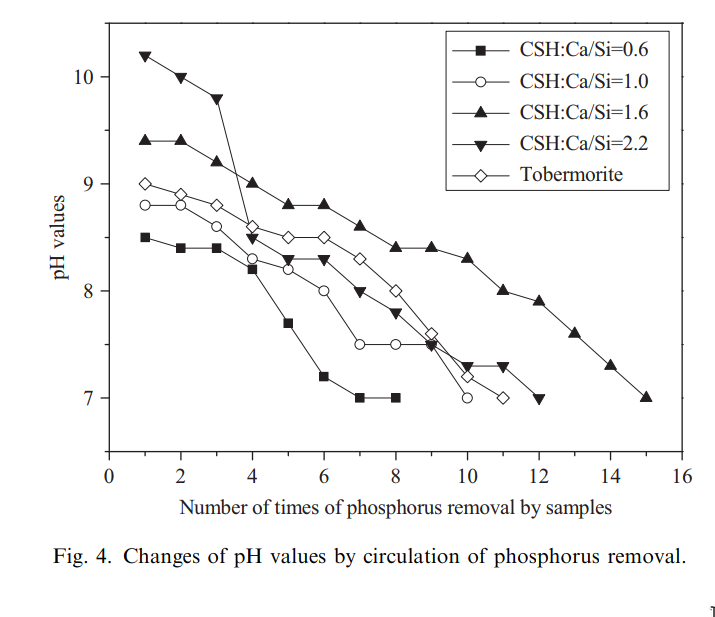
\includegraphics[width=0.9\textwidth]{fig.4.png} % first figure itself
        \caption{除磷循环对pH值的影响}
    \end{minipage}\hfill
    \begin{minipage}{0.45\textwidth}
        \centering
        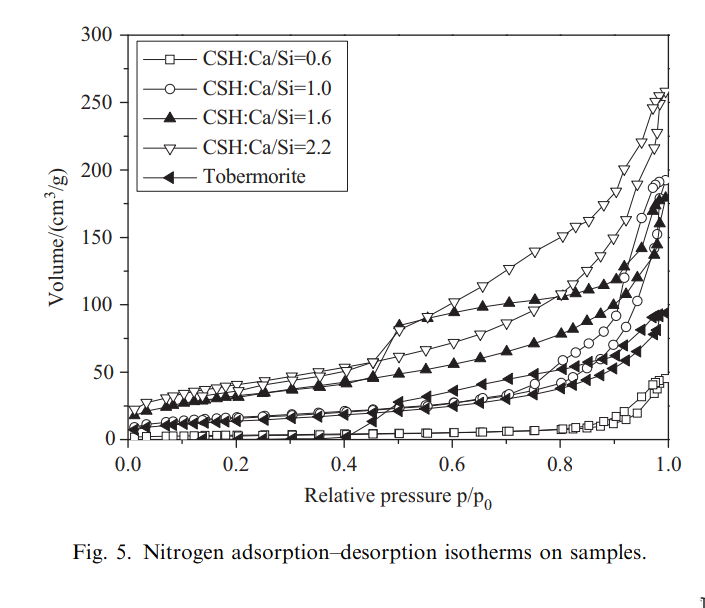
\includegraphics[width=0.9\textwidth]{fig.5.png} % second figure itself
        \caption{样品上的氮吸附 - 解吸等温线。}
    \end{minipage}
\end{figure}



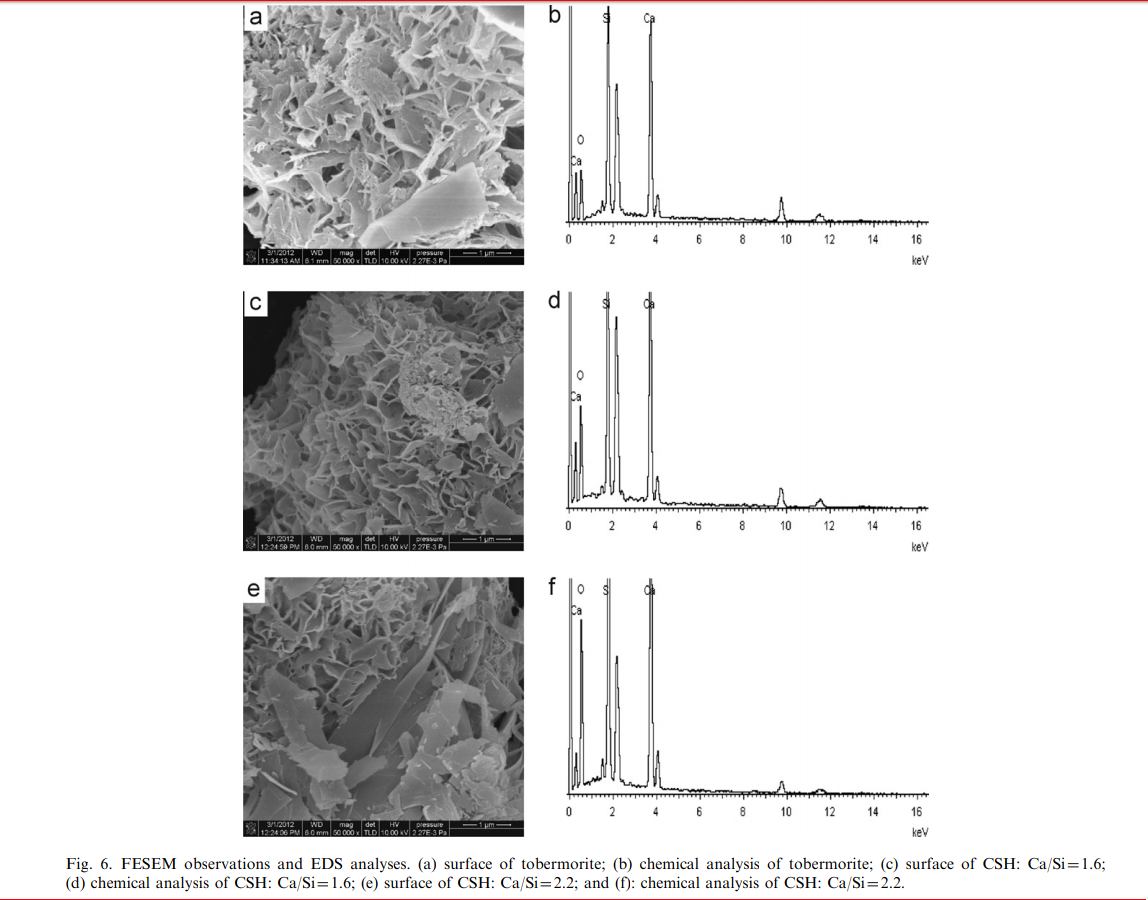
\includegraphics[width=0.9\textwidth]{fig.6.png}
\captionof{figure}{FESEM观察和EDS分析} \label{tab:title}

(a)雪硅钙石表面;
(b)雪硅钙石的化学分析;
(c)CSH表面: Ca/Si = 1.6;
(d)CSH的化学分析: Ca/Si = 1.6;
(e)CSH表面: Ca/Si = 2.2;
(f)CSH的化学分析:Ca/Si = 2.2;

\noindent\rule{\textwidth}{0.5pt}


\subsection{Ca\textsuperscript{2+}释放动力学}
\label{sec:org0e03bc0}
\setlength{\parindent}{1.0cm}
实验表明,Ca\textsuperscript{2+}浓度随着Ca/Si摩尔比的增加而增加(图7)。从雪硅钙石释放的
Ca\textsuperscript{2+}浓度,CSH: Ca/Si = 1.6和CSH: Ca/Si = 2.2分别为2.10, 3.56, 4.91mg/g。
根据Avrami动力学模型方程(方程(2)绘制Ca\textsuperscript{2+}释放的实验能力)。cite:demirkıran07\textsubscript{dissol}\textsubscript{kinet}\textsubscript{ulexit}\textsubscript{perch}\textsubscript{acid}\textsubscript{solut}
\par

\[-\ln(1-x) = kt^{n} \ \ \ (2)\]

\setlength{\parindent}{1.0cm}
其中k是动力学常数,n是固体的特征常数,t是反应时间(min)和x(x¼Ct/ C\textsubscript{max},Ct是时间t的浓度(mg/L),C\textsubscript{max}是最大浓度(mg)/L))是分数转换。特征常数n为0.9019。通过将Avrami动力学模型拟合到从图6(表2)获得的实验数据来确定动力学常数。高相关系数(R2> 0.99)表明该模型可以很好地描述Ca\textsuperscript{2+}释放规律。
\par


\setlength{\parindent}{1.0cm}
如表2所示,随着Ca/Si摩尔比的增加,k变大。结合材料的比表面积(S),可以建立k和S之间的关系(方程(3))。
\par

\[k = 0.022S^{0.292} \ \ R = 0.9135 \ \ \ (3)\]

\setlength{\parindent}{1.0cm}
根据方程(3)样品的比表面积和Ca\textsuperscript{2+}释放速率相互吻合良好。通过用方程(3)代替,得到比表面积与Ca\textsuperscript{2+}溶解浓度之间的关系进入方程(2)。
\par

\[-\ln(1-x) = 0.022S^{0.292}t^{0.9019} \ \ \ (4)\]

\setlength{\parindent}{1.0cm}
根据方程(4),Ca\textsuperscript{2+}释放浓度与比表面积有关。该结果证明了Ca/Si摩尔比对磷回收能力的影响。Ca/Si摩尔比影响孔结构和Ca\textsuperscript{2+}释放能力。由于比表面积较大,Ca\textsuperscript{2+}释放得更快。多孔结构提供了维持高浓度Ca\{2+\}释放的局部条件。比较CSH: Ca/Si = 1.6与CSH: Ca/Si = 2.2,前者具有较高的磷回收性能。因此,Ca\textsuperscript{2+}释放规律是磷回收性能的关键。CSH: Ca/Si = 1.6可以释放适当浓度的Ca\textsuperscript{2+}和OH\textsuperscript{-}以维持pH值在8.5-9.5之间。磷酸盐以这些pH值范围内的HPO\textsuperscript{2-}\textsubscript{4}形式存在.cite:liu12\textsubscript{remov}\textsubscript{high}\textsubscript{concen}\textsubscript{phosp}\textsubscript{by}\textsubscript{calcit} Ca\textsuperscript{2+},OH\textsuperscript{-}和HPO\textsuperscript{2-}\textsubscript{4}形成高浓度的局部条件。这种条件(pH = 8.5-9.5)有利于羟基磷灰石的形成。
\par

\setlength{\parindent}{1.0cm}
可以通过XRD进一步研究该机理。比较样品的XRD图谱(图8)。当Ca/Si摩尔比为0.6:1和1:1时,
生产硬硅钙石(PDF卡23 0125,化学式Ca\textsubscript{6}Si\textsubscript{6}O\textsubscript{17}(OH)\textsubscript{2})。对于CSH: Ca/Si =
0.6,SiO 2的主峰出现在20.3051和21.5621。CSH中的主峰: Ca/Si = 1.6和CSH: Ca/Si = 2.2
归属于jennite(PDF卡18-1206;式Ca\textsubscript{9}Si\textsubscript{6}O\textsubscript{18}(OH)\textsubscript{6}·8H\textsubscript{2}O;理论Ca/Si摩尔比
为1.5)。CSH: Ca/Si = 2.2的XRD图谱显示存在Ca(OH)\textsubscript{2}。形成的Ca(OH)\textsubscript{2}的覆盖率与基于FESEM观察的结果完全一致[27]。
\par

\begin{figure}
    \centering
    \begin{minipage}{0.45\textwidth}
        \centering
        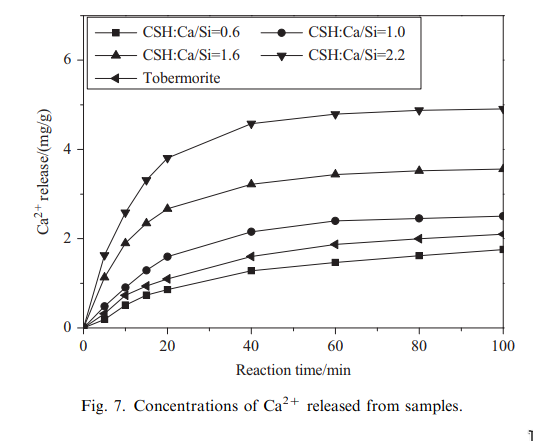
\includegraphics[width=0.9\textwidth]{fig.7.png} % first figure itself
        \caption{样品中释放的Ca^{2+}浓度}
    \end{minipage}\hfill
    \begin{minipage}{0.45\textwidth}
        \centering
        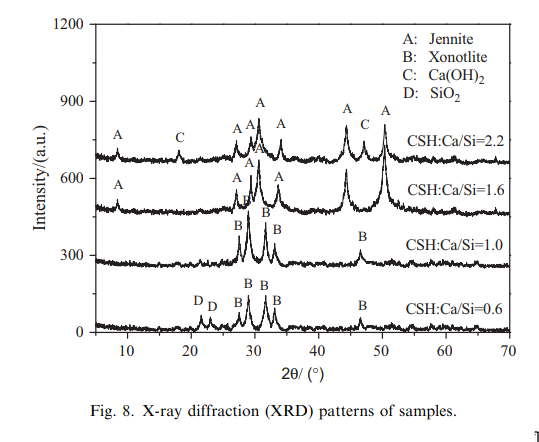
\includegraphics[width=0.9\textwidth]{fig.8.png} % second figure itself
        \caption{样品的X射线衍射(XRD)图案。}
    \end{minipage}
\end{figure}

\setlength{\parindent}{1.0cm}
实验表明,与硬硅钙石和雪硅钙石相比,jennite具有更强的Ca\textsuperscript{2+}释放能力。低Ca/Si
摩尔比导致白炭黑过剩。因此,在材料表面上形成富含Si的层并阻止Ca\textsuperscript{2+}释放。随后,
材料的磷回收能力下降。Ca(OH)\textsubscript{2}的形成是由于具有高Ca/Si摩尔比的碳化物残余物的
过剩。由于Ca(OH)\textsubscript{2}的存在,CSH的单磷去除效率: Ca/Si = 2.2优于其他样品。然而,
大量的Ca\textsuperscript{2+}被释放并与浸入合成溶液中的材料一样快地与磷酸根离子反应。羟基磷灰石层在短时间内形成并导致孔结构的阻塞。因此Ca\textsuperscript{2+}释放能力下降。
\par

\section{总结}
\label{sec:orgfe1cc80}

bibliography:man.bib
bibliographystyle:ieeetr
\end{document}
